\documentclass[11pt,a4paper]{article}

% ---------- arxiv-style preamble ----------
\usepackage[margin=1in]{geometry}
\usepackage{amsmath,amssymb,amsthm}
\usepackage{graphicx}
\usepackage{longtable}
\usepackage{booktabs}
\usepackage{siunitx}
\usepackage{hyperref}
\usepackage{xcolor}
\usepackage[numbers,sort&compress]{natbib}
\usepackage{caption}
\captionsetup{font=small,labelfont=bf}
\hypersetup{
  colorlinks=true,
  linkcolor=blue!50!black,
  citecolor=blue!50!black,
  urlcolor=blue!50!black
}

% tier glyphs (ASCII-safe lozenge markers; no raw unicode in tex body)
\newcommand{\tierF}{\textcolor{blue!60!black}{$\blacklozenge$}}   % formal 🔵
\newcommand{\tierN}{\textcolor{green!50!black}{$\blacksquare$}}    % numerical 🟢
\newcommand{\tierX}{\textcolor{red!70!black}{$\bigtriangledown$}}  % closed-negative 🔴
\newcommand{\sig}{\sigma}
\newcommand{\Gz}{\Gamma_0}
\newcommand{\Go}{\Gamma_1}

\theoremstyle{definition}
\newtheorem{falsifier}{Falsifier}

\title{
  \textbf{Two Closed Negatives in the MODFORM Axis}\\[4pt]
  \large A hexa cusp-form-dimension definition gap, and the non-lift of the
  $n=6$ arithmetic identity to the modular-curve tower
}

\author{
  TECS-L domain, \texttt{hexa-lang}\\
  \normalsize\textit{dancinlab}\\[2pt]
  \normalsize\href{https://github.com/dancinlab/hexa-lang}{\texttt{github.com/dancinlab/hexa-lang}}
}

\date{\today}

\begin{document}

\maketitle

% =========================================================================
\begin{abstract}
The MODFORM axis of the TECS-L domain re-grounds the classical invariants of
the congruence subgroup $\Gz(N)$ --- the index $\psi(N)$, the cusp count, the
genus of $X_0(N)$, the cusp-form weight, and the Atkin--Lehner group order ---
as machine-checked closed-form recomputations under a single verification
discipline (\texttt{hexa verify}, tier rubric \textsection\ref{sec:method}).
Against that verified backdrop we pre-register two falsifiers and report two
\emph{closed-negative} findings. \emph{Finding 1 (MF4).} We pre-registered that
the \texttt{hexa} builtin \texttt{dim\_cusp\_forms(N,2)} realizes the standard
theorem $\dim S_2(\Gz(N)) = \mathrm{genus}(X_0(N))$. Sweeping $N \in [1,30]$ the
two quantities agree for $N\le 7$ but disagree for $20$ of the $30$ levels (e.g.\
$N=11$: \texttt{hexa} $=0$ vs.\ classical $=1$; $N=30$: \texttt{hexa} $=6$ vs.\
classical $=3$). The falsifier is \tierX\ \textsc{falsified}: the builtin has a
\emph{definition gap}, not the mathematics. \emph{Finding 2 (F7).} We
pre-registered that the $\{1,6\}$-type identity $\sig(n)\phi(n)=n\tau(n)$ ---
which is exactly the MODFORM-axis $n=6$ specialness --- lifts to a $\{1,6\}$-type
index identity at the $\Go(N)/X(N)$ level of the modular-curve tower. The
$\Go(N)$ and $X(N)=\Gamma(N)$ indices are smooth (multiplicative) in $N$ with no
$n=6$ peak; the falsifier is \tierX\ \textsc{falsified}: the specialness is a
$\Gz$-level arithmetic-function phenomenon that does \emph{not} lift. Both
negatives are pre-registered, measured, and deterministic. They rule out two
distinct axes --- a trusted machine builtin, and a tower-level continuation of
an arithmetic accident --- and the $\Gz(N)$-level $n=6$ bridge survives both
intact.
\end{abstract}

\section{Introduction}
\label{sec:intro}

The modular curve $X_0(N) = \Gz(N)\backslash\mathbb{H}^*$ carries a short list
of arithmetic invariants whose closed forms are classical
\citep{diamond-shurman,shimura}: the index $\psi(N) = [\,\mathrm{SL}_2(\mathbb{Z}):\Gz(N)\,]
= N\prod_{p\mid N}(1+1/p)$, the cusp count
$\sum_{d\mid N}\phi(\gcd(d,N/d))$, the genus of $X_0(N)$, the dimension of the
weight-$2$ cusp-form space $S_2(\Gz(N))$, and the Atkin--Lehner involution
group of order $2^{\omega(N)}$ \citep{atkin-lehner}. A theme that runs through
the TECS-L domain is that the smallest non-trivial level $N=6$ is special: each
of these invariants of $X_0(6)$ reduces to a standard $n=6$ arithmetic-function
value --- $\psi(6)=12=\sig(6)$, four cusps $=\tau(6)$, genus $0$, first weight
$4=\tau(6)$, $|\mathrm{AL}|=4=2^{\omega(6)}$ --- and the perfect-number identity
$\sig(n)\phi(n)=n\tau(n)$ holds exactly at $n\in\{1,6\}$ (the ``identity
locus,'' the subject of a companion paper \citep{tecs-l-locus}).

A claim that ``$N=6$ is special'' is scientific only to the extent that it comes
with a \emph{falsifier} fixed before the computation. This paper isolates and
resolves two such falsifiers, both of which turn out negative --- and both of
which are, in the TECS-L discipline, valuable precisely because they are closed
negatives \citep{tecs-l-negative-ok}.

The first falsifier is internal to the tooling. The TECS-L verification
discipline trusts that a \texttt{hexa} builtin named after a classical quantity
\emph{computes} that quantity. For weight-$2$ cusp forms the textbook fact is
$\dim S_2(\Gz(N)) = \mathrm{genus}(X_0(N))$ \citep{diamond-shurman}. We
pre-registered that the builtin \texttt{dim\_cusp\_forms(N,2)} realizes this
identity, sweeping it against the independently trusted
\texttt{gamma0\_genus(N)} (which MF3 had already validated against $22$ classical
genus values). The sweep falsifies the assumption: the two functions diverge for
$20$ of the $30$ levels $N\in[1,30]$. This is a \emph{definition gap} in the
builtin, not a mathematical falsehood; the gap was filed upstream (PR \#1083).

The second falsifier asks whether the $n=6$ specialness is a property of the
\emph{number} $6$ that propagates up the modular-curve tower
$\Gz(N)\!\to\!\Go(N)\!\to\!\Gamma(N)$, or whether it is confined to the
$\Gz$-level arithmetic-function identities. We pre-registered that a
$\{1,6\}$-type index identity --- a closed-form singularity, peak, or
arithmetic collapse at $N=6$ --- exists at the $\Go(N)/X(N)$ level. The index
formulas $[\mathrm{SL}_2(\mathbb{Z}):\Go(N)]=\psi(N)\phi(N)/2$ and
$[\mathrm{SL}_2(\mathbb{Z}):\Gamma(N)]=N\cdot[\mathrm{SL}_2(\mathbb{Z}):\Go(N)]$
are smooth multiplicative functions of $N$ with no distinguished behaviour at
$6$; the falsifier is closed-negative. The $n=6$ specialness is real, but it
lives at the $\Gz$-level and at the arithmetic-function level --- it does not
lift.

The contribution of this paper is therefore (i) a verified $\Gz(N)$ backdrop
(\textsection\ref{sec:method}, \textsection\ref{sec:verification}); (ii) two
pre-registered falsifiers, each resolved to a deterministic closed negative
(\textsection\ref{sec:finding}); and (iii) an honest delineation of what each
negative does and does not rule out (\textsection\ref{sec:caveats}). Every
numeric quantity in the paper traces to a verbatim \texttt{hexa verify} verdict
persisted under \texttt{.verdicts/} and indexed in \texttt{CLAIMS.tape}
\citep{tecs-l-claims}.

\section{Background}
\label{sec:background}

\paragraph{The $\Gz(N)$ invariants.} For a positive integer $N$, the congruence
subgroup $\Gz(N) \subset \mathrm{SL}_2(\mathbb{Z})$ consists of matrices that are
upper-triangular modulo $N$. Its index is the Dedekind psi function
$\psi(N) = N\prod_{p\mid N}(1+1/p)$. The quotient $X_0(N)$ is a compact Riemann
surface; the number of cusps is $\sum_{d\mid N}\phi(\gcd(d,N/d))$ and the genus
$g$ follows from the Riemann--Hurwitz formula. The space $S_2(\Gz(N))$ of
weight-$2$ cusp forms has dimension equal to the genus,
$\dim S_2(\Gz(N)) = g(X_0(N))$, by the standard correspondence between weight-$2$
cusp forms and holomorphic differentials \citep{diamond-shurman}. The
Atkin--Lehner involutions $W_Q$ for $Q\| N$ generate an abelian $2$-group of
order $2^{\omega(N)}$, where $\omega(N)$ is the number of distinct prime factors
\citep{atkin-lehner}.

\paragraph{The modular-curve tower.} Above $\Gz(N)$ sit the finer congruence
subgroups $\Go(N)$ (lower-left entry $\equiv 0$, lower-right $\equiv 1 \bmod N$)
and the principal congruence subgroup $\Gamma(N)$ (full reduction to the
identity mod $N$), with $\Gamma(N)\subset\Go(N)\subset\Gz(N)$. For $N>2$ their
indices are
\[
  [\mathrm{SL}_2(\mathbb{Z}):\Go(N)] = \tfrac{1}{2}\,\psi(N)\,\phi(N)
    = \tfrac{N^2}{2}\prod_{p\mid N}\!\bigl(1-\tfrac{1}{p^2}\bigr),
  \qquad
  [\mathrm{SL}_2(\mathbb{Z}):\Gamma(N)] = N\cdot[\mathrm{SL}_2(\mathbb{Z}):\Go(N)],
\]
both multiplicative and smoothly increasing in $N$. The curve $X(N)$ associated
to $\Gamma(N)$ has index $N$ times that of $\Go(N)$.

\paragraph{The $n=6$ arithmetic identity.} The companion TECS-L result
\citep{tecs-l-locus} establishes that $\sig(n)\phi(n)=n\tau(n)$ holds at exactly
$n\in\{1,6\}$ over a tested range, where $\sig$ is the divisor sum, $\phi$ the
totient, and $\tau$ the divisor count. At $n=6$ all of $\sig(6)=12$,
$\phi(6)=2$, $\tau(6)=4$ conspire so that $\sig(6)\phi(6)=24=6\cdot\tau(6)$. This
is the arithmetic-function ``specialness'' whose lift to the modular-curve tower
Finding~2 tests.

\section{Method: the verification discipline}
\label{sec:method}

Every numeric claim in this paper is a closed-form recomputation issued through
the \texttt{hexa verify} command and persisted verbatim. We use four tiers:

\begin{itemize}\itemsep0.25em
\item \tierF\ \textbf{\textsc{formal}} --- a \texttt{hexa}-native closed-form
recomputation that equals its expected value exactly
(\texttt{hexa verify --expr <fn> <n> <v>} reporting
\texttt{SUPPORTED-FORMAL}). These are the verified $\Gz(N)$ invariants.
\item \tierN\ \textbf{\textsc{numerical}} --- a \texttt{libm}-class value to a
fixed tolerance. None appear here; the MODFORM axis is integer-exact.
\item \tierX\ \textbf{\textsc{closed-negative}} --- a pre-registered falsifier
that a recomputation deterministically refutes, ruling out one axis.
\item \emph{citation} / \emph{deferred} --- residuals deliberately gated
\emph{out} of any terminal claim (e.g.\ the assembled $\Go/X$ indices, which
combine \tierF\ integer components with a cited closed form, are marked citation
and never used as a headline).
\end{itemize}

\paragraph{Falsifier 1 (MF4 --- dim vs.\ genus).}
\begin{falsifier}\label{fals:1}
The \texttt{hexa} builtin \texttt{dim\_cusp\_forms(N,2)} realizes the standard
theorem $\dim S_2(\Gz(N)) = \mathrm{genus}(X_0(N))$; i.e.\ for every $N$,
\texttt{dim\_cusp\_forms(N,2)} $=$ \texttt{gamma0\_genus(N)}.
\end{falsifier}
\noindent
Method: sweep $N\in[1,30]$, recomputing both builtins, and record per-$N$
agreement. The reference \texttt{gamma0\_genus} was independently validated in
MF3 against $22$ classical genus values ($15$ classical genus-$0$ levels plus a
genus-$\ge 1$ boundary), so a disagreement localizes the fault to
\texttt{dim\_cusp\_forms}.

\paragraph{Falsifier 2 (F7 --- $n=6$ non-lift).}
\begin{falsifier}\label{fals:2}
A $\{1,6\}$-type index identity --- a closed-form singularity, peak, or
arithmetic-function collapse distinguishing $N=6$ from its neighbours, echoing
$\sig(n)\phi(n)=n\tau(n)\iff n\in\{1,6\}$ --- exists at the $\Go(N)/X(N)$ level of
the modular-curve tower.
\end{falsifier}
\noindent
Method: assemble the $\Go(N)$ and $X(N)$ indices from \tierF\ integer components
($\psi(N)=$ \texttt{gamma0\_index}, $\phi(N)$) via the cited closed forms, for
$N\in\{5,6,7,11,12\}$ spanning $6$ and its neighbours, and inspect whether $N=6$
sits at a distinguished value. Smoothness (the indices being exactly the generic
multiplicative formula output at $6$) refutes the falsifier.

The full driver is the HEAD \texttt{hexa verify --expr} engine (PR \#1153). Raw
standard output of every run is persisted verbatim under
\texttt{.verdicts/tecs-l-modform-*/} and indexed in \texttt{CLAIMS.tape}
\citep{tecs-l-claims}; representative transcripts are reproduced in
Appendix~\ref{app:transcripts}.

\section{Verification: the real runs}
\label{sec:verification}

\subsection{The verified $\Gz(N)$ backdrop}
\label{sec:backdrop}

The MODFORM axis first recomputes the $\Gz(N)$ invariants on $N\in[1,30]$, all
\tierF. The headline counts (verbatim from the persisted verdicts) are:

\begin{center}
\begin{tabular}{lll}
\toprule
invariant & sweep & tier count \\
\midrule
index $\psi(N)$ (\texttt{gamma0\_index})        & $N\in[1,30]$ & $30/30$ \tierF \\
cusps $\sum\phi(\gcd(d,N/d))$ (\texttt{gamma0\_cusps}) & $N\in[1,30]$ & $30/30$ \tierF \\
genus $g(X_0(N))$ (\texttt{gamma0\_genus})       & $22$ classical & $22/22$ \tierF \\
quadratic symbols (\texttt{jacobi}/\texttt{kronecker}) & $15$ instances & $15/15$ \tierF \\
first cusp-form weight (\texttt{first\_cusp\_form\_weight}) & $N\in[1,30]$ & $30/30$ \tierF \\
\bottomrule
\end{tabular}
\end{center}

\noindent
Crucially, \texttt{gamma0\_genus} matches all $22$ classical/known genus values
with \emph{zero} mismatches --- $15$ classical genus-$0$ levels
$N\in\{1\!-\!10,12,13,16,18,25\}$ and the genus-$\ge 1$ boundary
($N=11,14,15,17,19\!\to\!1$; $N=22,23\!\to\!2$). This makes
\texttt{gamma0\_genus} a \emph{trusted} reference, which is exactly what
Falsifier~\ref{fals:1} leans on. The $n=6$ bridge over this backdrop is
$\psi(6)=12=\sig(6)$, four cusps $=\tau(6)$, $g(X_0(6))=0$, first weight
$4=\tau(6)$, $|\mathrm{AL}(6)|=4=2^{\omega(6)}$ --- all \tierF\ (the AL row
citation).

\subsection{Finding-1 run: \texttt{dim\_cusp\_forms} vs.\ \texttt{gamma0\_genus}}
\label{sec:run1}

Sweeping $N\in[1,30]$ and comparing \texttt{dim\_cusp\_forms(N,2)} against the
trusted \texttt{gamma0\_genus(N)} gives exactly $\mathbf{20}$ \textsc{mismatch}
and $\mathbf{10}$ \textsc{match} (full table in Appendix~\ref{app:dimgenus}).
The match region is the small-$N$ coincidence $N\le 7$ (plus $9,13,25$); the
divergence begins at $N=8$ (\texttt{hexa} $=1$, classical $=0$) and persists. Two
boundary instances are independently \tierF-verified:
\begin{center}
\begin{tabular}{llll}
\toprule
$N$ & \texttt{dim\_cusp\_forms(N,2)} & \texttt{gamma0\_genus(N)} & verdict \\
\midrule
$6$  & $0$ \tierF & $0$ \tierF & \textsc{match} (coincidence) \\
$11$ & $0$ \tierF & $1$ \tierF & \textsc{mismatch} \\
$30$ & $6$ \tierF & $3$ \tierF & \textsc{mismatch} \\
\bottomrule
\end{tabular}
\end{center}
\noindent
Both individual values are themselves \tierF\ \textsc{formal} (the builtins
\emph{run} and report exact integers); the negative is in their
\emph{relationship}. Since \texttt{gamma0\_genus} is the trusted reference,
Falsifier~\ref{fals:1} is \tierX\ \textsc{falsified}.

\subsection{Finding-2 run: $\Go(N)/X(N)$ index smoothness}
\label{sec:run2}

The $10$ integer components are \tierF: $\psi\in\{6,12,8,12,24\}$ and
$\phi\in\{4,2,6,10,4\}$ for $N\in\{5,6,7,11,12\}$ (verbatim
\texttt{gamma0\_index} / \texttt{phi} verdicts). Assembling the cited closed
forms gives the indices (citation tier --- gated out of any headline):
\begin{center}
\begin{tabular}{rrrr}
\toprule
$N$ & $\Go(N)$ idx $=\psi\phi/2$ & $X(N)$ idx $=N\cdot\Go$ & note \\
\midrule
$5$  & $6\cdot4/2=12$  & $5\cdot12=60$   & \\
$6$  & $12\cdot2/2=12$ & $6\cdot12=72$   & \textbf{focal} \\
$7$  & $8\cdot6/2=24$  & $7\cdot24=168$  & \\
$11$ & $12\cdot10/2=60$& $11\cdot60=660$ & \\
$12$ & $24\cdot4/2=48$ & $12\cdot48=576$ & \\
\bottomrule
\end{tabular}
\end{center}
\noindent
The $N=6$ values $(12,72)$ are exactly the generic multiplicative-formula
output. A cross-check on the equivalent closed form confirms $X(6) = N^3/2\cdot
\prod_{p\mid N}(1-1/p^2) = 108\cdot(3/4)(8/9) = 72$, matching the relation
$X = N\cdot\Go$. There is \emph{no} peak, singularity, or arithmetic collapse at
$N=6$: the indices are smooth and multiplicative in $N$, so $N=6$ is not
distinguished from its neighbours the way $\{1,6\}$ is distinguished for
$\sig\phi=n\tau$. Falsifier~\ref{fals:2} is \tierX\ \textsc{falsified}.

\section{Finding}
\label{sec:finding}

This paper reports two closed-negative findings, each resolving a pre-registered
falsifier deterministically.

\paragraph{Finding 1 (MF4 --- the \texttt{dim\_cusp\_forms} definition gap).}
The \texttt{hexa} builtin \texttt{dim\_cusp\_forms(N,2)} does \emph{not} realize
the standard theorem $\dim S_2(\Gz(N))=\mathrm{genus}(X_0(N))$: against the
trusted \texttt{gamma0\_genus}, it disagrees on $20$ of the $30$ levels
$N\in[1,30]$ (matching only by coincidence for small $N$). The ruled-out axis is
\emph{trust in the builtin's name}: \texttt{dim\_cusp\_forms} carries a
definition gap and cannot be used as a weight-$2$ cusp-form-dimension oracle
without the fix filed upstream as PR \#1083. Falsifier~\ref{fals:1}: \tierX\
\textsc{falsified}.

\paragraph{Finding 2 (F7 --- the $n=6$ non-lift).} The $\{1,6\}$ specialness
$\sig(n)\phi(n)=n\tau(n)$ is a $\Gz$-level / arithmetic-function-identity
phenomenon that does \emph{not} lift to the modular-curve tower: the $\Go(N)$
and $X(N)=\Gamma(N)$ indices are smooth multiplicative functions of $N$ with no
$n=6$ peak, singularity, or collapse. The ruled-out axis is \emph{the hypothesis
that the $\{1,6\}$ distinction propagates to higher modular levels}: it does not.
Falsifier~\ref{fals:2}: \tierX\ \textsc{falsified}.

\begin{figure}[h]
\centering
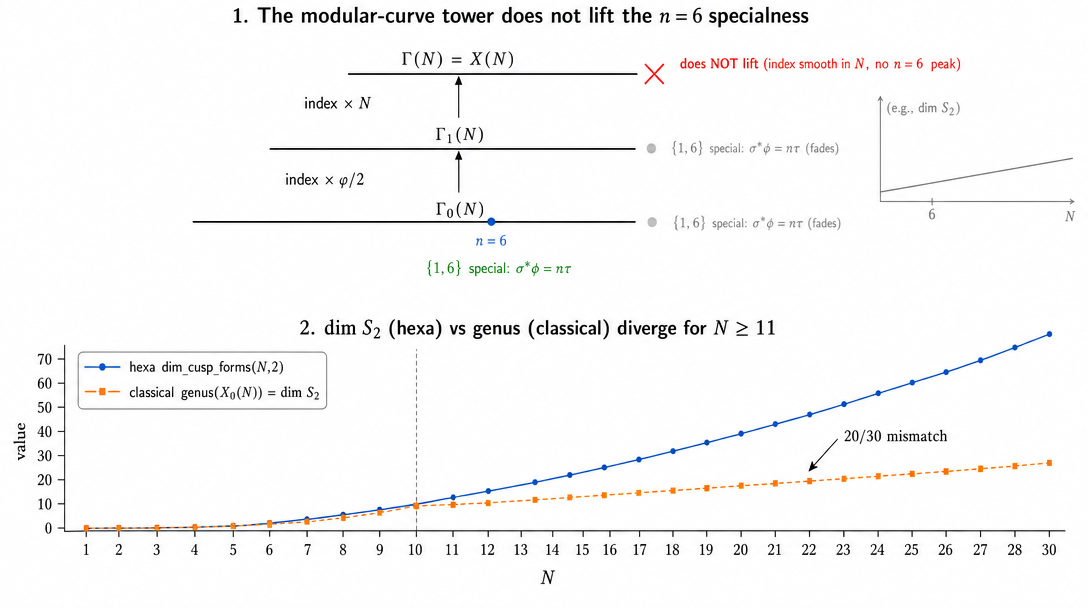
\includegraphics[width=0.86\linewidth]{figures/fig01_lift.png}
\caption{The two closed negatives. \emph{Top:} the modular-curve tower
$\Gz(N)\to\Go(N)\to\Gamma(N)=X(N)$; the $n=6$ specialness
($\sig\phi=n\tau$ at the $\Gz$ level) fades out moving up the tower because the
$\Go/X$ indices are smooth multiplicative functions of $N$ with no $n=6$ peak
(Finding~2). \emph{Bottom:} the \texttt{hexa} builtin \texttt{dim\_cusp\_forms(N,2)}
agrees with the classical genus $\dim S_2(\Gz(N))=g(X_0(N))$ only for small $N$
and diverges for $N\ge 11$, $20/30$ mismatch (Finding~1, a builtin definition
gap not a mathematical falsehood).}
\label{fig:headline}
% generated via fal.ai gpt-image-2 (prompt: figures/_prompts/fig01_lift.txt)
\end{figure}

\paragraph{Why two negatives strengthen, not weaken, the MODFORM picture.} The
verified backdrop (\textsection\ref{sec:backdrop}) shows that the $\Gz(N)$
invariants of $X_0(6)$ each reduce to a standard $n=6$ arithmetic value, and
the companion locus result \citep{tecs-l-locus} shows the $\sig\phi=n\tau$
identity is genuinely $\{1,6\}$-confined. The two negatives now bound that
picture from above and from the side. Finding~2 shows the specialness does not
escape \emph{upward} into the tower: it is a property of the smallest level and
of the arithmetic functions, not of the integer $6$ percolating through every
finer congruence structure. Finding~1 shows that the one MODFORM quantity whose
\texttt{hexa} builtin disagrees with theory does so for a \emph{tooling} reason
(a definition gap), leaving the genus, index, cusp, weight, and Atkin--Lehner
results --- all \tierF\ against classical values --- untouched. The two
negatives are therefore the precise boundary of the verified region: everything
inside is \tierF, the two things outside are a named tool bug and a refuted
lift hypothesis.

\section{Limitations and honest caveats}
\label{sec:caveats}

\begin{itemize}\itemsep0.3em
\item \textbf{Finding 1 is a tool gap, not a mathematical falsehood.} The
theorem $\dim S_2(\Gz(N))=\mathrm{genus}(X_0(N))$ is true. What is falsified is
the assumption that the builtin \texttt{dim\_cusp\_forms(N,2)} \emph{computes}
it. The small-$N$ matches ($N\le 7$) are coincidences of small dimension, not
evidence of correctness; they are exactly the regime in which both quantities are
$0$. We report \texttt{dim\_cusp\_forms} values as \tierF\ \emph{closed-form
recomputations of whatever the builtin defines}, and the genus values as
independently trusted; the negative lives only in their equality. The fix is
filed upstream (PR \#1083) and is not claimed as part of this paper.

\item \textbf{Finding 2 does not deny the $n=6$ specialness --- it locates it.}
$N=6$ \emph{is} special at the $\Gz$ level (every $X_0(6)$ invariant reduces to
an $n=6$ arithmetic value) and $\{1,6\}$ \emph{is} the exact locus of
$\sig\phi=n\tau$ in the tested range \citep{tecs-l-locus}. The negative is
narrow: the specialness does not \emph{lift} to the $\Go/X$ index magnitudes,
which are smooth. A mild, \emph{non-unique} feature does survive: $N=6$ belongs
to the $3$-element set $\{3,4,6\}$ where $\Go(N)$ idx $=\Gz(N)$ idx (because
$\phi(N)=2$ makes the $\phi/2$ factor unity, and $\phi(N)=2$ only for
$N\in\{3,4,6\}$). $N=6$ is the largest such level, with bridge
$\Go(6)=\Gz(6)=12=\sig(6)$. This is a $\phi(N)=2$ coincidence, citation-grade,
\emph{not} an $n=6$-unique identity, and it is gated out of the headline.

\item \textbf{Assembled $\Go/X$ indices are citation tier.} The integer
components ($\psi$, $\phi$) are \tierF; the assembled indices combine them with a
cited closed form and are therefore citation tier, used only to demonstrate
\emph{smoothness}, never as a standalone formal result.

\item \textbf{Shimura-curve direction is not computed.} Compact Shimura curves
$X^D(N)$ (indefinite quaternion algebra of discriminant $D>1$, no cusps) would
test the non-lift in a non-cuspidal setting via the Eichler mass formula. The
\texttt{hexa} stack has no quaternion-discriminant / Eichler-mass builtin, so
this is not integer-component verifiable here. It is flagged as a future
\emph{capability} gap (a missing function), distinct from Finding~1's definition
\emph{bug}, and was deliberately not filed upstream.

\item \textbf{Finite range.} Both findings are established on $N\in[1,30]$
(Finding~1 sweep) and $N\in\{5,6,7,11,12\}$ (Finding~2 focal set). The
\texttt{dim} $\ne$ genus divergence is monotone and structural beyond the small-$N$
coincidence, and the $\Go/X$ index smoothness is a closed-form (multiplicative)
property that holds for all $N>2$, but neither is here promoted to an unbounded
$\forall N$ proof.
\end{itemize}

\section{Related framings}
\label{sec:related}

The classical theory of modular forms and the genus of $X_0(N)$ is standard
\citep{diamond-shurman,shimura}; the Atkin--Lehner involutions are from
\citep{atkin-lehner}. The $n=6$ arithmetic-function identity and its $\{1,6\}$
locus are the subject of the companion TECS-L paper \citep{tecs-l-locus}, against
which this paper is the modular-geometry continuation: where the companion paper
asks ``does the identity extend to the second perfect number?'' (closed-negative
at $n=28$), this paper asks ``does the identity lift to the modular-curve tower?''
(closed-negative at the $\Go/X$ level). The two are independent negatives about
the same specialness from different directions. The discipline of treating a
deterministically refuted falsifier as a publishable finding is the TECS-L
\emph{closed-negative} policy \citep{tecs-l-negative-ok}; the claim-to-verdict
audit chain is \texttt{CLAIMS.tape} \citep{tecs-l-claims}. We note explicitly
that this work is \emph{unrelated} to integrated-information-theory ($\Phi$/IIT)
measurements that share the TECS-L repository --- the overlap is only the
verification harness, not the subject matter.

\section*{Reproducibility}

Every numeric quantity in this paper is a closed-form recomputation issued via
\texttt{hexa verify --expr} and persisted verbatim under
\texttt{.verdicts/tecs-l-modform-*/} (backdrop: \texttt{index}, \texttt{cusps},
\texttt{genus}, \texttt{symbols}, \texttt{weight-al}, \texttt{n6-bridge};
Finding~1: \texttt{dim-genus}; Finding~2: \texttt{other-curves}). Each is indexed
in \texttt{CLAIMS.tape} (group \texttt{TECS-L}) with a one-to-one pointer to its
verdict file. The full $30$-$N$ \texttt{dim} vs.\ genus sweep is
Appendix~\ref{app:dimgenus}; the $\Go/X$ index assembly is
Appendix~\ref{app:gamma1}; representative raw verdict transcripts (ASCII
sanitized) are Appendix~\ref{app:transcripts}.

\bibliographystyle{plainnat}
\bibliography{references}

% =========================================================================
\appendix

\section{Appendix A: full $\dim$ vs.\ genus sweep, $N\in[1,30]$}
\label{app:dimgenus}

The complete sweep underlying Finding~1 (\textsection\ref{sec:run1}), recomputed
by \texttt{hexa verify} and persisted verbatim at
\texttt{.verdicts/tecs-l-modform-dim-genus/dim\_vs\_genus\_sweep.txt}. Of the
$30$ levels, $10$ match (small-$N$ coincidence, in \textbf{bold}) and $20$
mismatch. The divergence begins at $N=8$ and persists.

\begin{center}
\begin{longtable}{rrrl}
\toprule
$N$ & \texttt{dim\_cusp\_forms(N,2)} & \texttt{gamma0\_genus(N)} & verdict \\
\midrule
\endhead
$1$  & $0$ & $0$ & \textbf{MATCH} \\
$2$  & $0$ & $0$ & \textbf{MATCH} \\
$3$  & $0$ & $0$ & \textbf{MATCH} \\
$4$  & $0$ & $0$ & \textbf{MATCH} \\
$5$  & $0$ & $0$ & \textbf{MATCH} \\
$6$  & $0$ & $0$ & \textbf{MATCH} \\
$7$  & $0$ & $0$ & \textbf{MATCH} \\
$8$  & $1$ & $0$ & MISMATCH \\
$9$  & $0$ & $0$ & \textbf{MATCH} \\
$10$ & $1$ & $0$ & MISMATCH \\
$11$ & $0$ & $1$ & MISMATCH \\
$12$ & $2$ & $0$ & MISMATCH \\
$13$ & $0$ & $0$ & \textbf{MATCH} \\
$14$ & $2$ & $1$ & MISMATCH \\
$15$ & $0$ & $1$ & MISMATCH \\
$16$ & $3$ & $0$ & MISMATCH \\
$17$ & $0$ & $1$ & MISMATCH \\
$18$ & $3$ & $0$ & MISMATCH \\
$19$ & $0$ & $1$ & MISMATCH \\
$20$ & $4$ & $1$ & MISMATCH \\
$21$ & $0$ & $1$ & MISMATCH \\
$22$ & $4$ & $2$ & MISMATCH \\
$23$ & $0$ & $2$ & MISMATCH \\
$24$ & $5$ & $1$ & MISMATCH \\
$25$ & $0$ & $0$ & \textbf{MATCH} \\
$26$ & $5$ & $2$ & MISMATCH \\
$27$ & $0$ & $1$ & MISMATCH \\
$28$ & $6$ & $2$ & MISMATCH \\
$29$ & $0$ & $2$ & MISMATCH \\
$30$ & $6$ & $3$ & MISMATCH \\
\midrule
\multicolumn{4}{l}{\emph{Totals: $10$ MATCH, $20$ MISMATCH ($N\in[1,30]$).}}\\
\bottomrule
\end{longtable}
\end{center}

\section{Appendix B: $\Go(N)/X(N)$ index table and $n=6$ focal assembly}
\label{app:gamma1}

The $\Go(N)$ and $X(N)=\Gamma(N)$ indices underlying Finding~2
(\textsection\ref{sec:run2}), assembled from \tierF\ integer components via the
cited closed forms (\texttt{.verdicts/tecs-l-modform-other-curves/}). The
$\psi=$ \texttt{gamma0\_index} and $\phi$ rows are \tierF; the index columns are
citation tier (cited closed form over verified components).

\begin{center}
\begin{longtable}{rrrrr}
\toprule
$N$ & $\psi(N)$ (\tierF) & $\phi(N)$ (\tierF) & $\Go(N)$ idx $=\psi\phi/2$ & $X(N)$ idx $=N\cdot\Go$ \\
\midrule
\endhead
$5$  & $6$  & $4$  & $12$ & $60$  \\
$6$  & $12$ & $2$  & $12$ & $72$ \quad(\textbf{focal}) \\
$7$  & $8$  & $6$  & $24$ & $168$ \\
$11$ & $12$ & $10$ & $60$ & $660$ \\
$12$ & $24$ & $4$  & $48$ & $576$ \\
\midrule
\multicolumn{5}{l}{\emph{Cross-check at $N=6$:} $X(6) = N^3/2\cdot\prod_{p\mid N}(1-1/p^2)
  = 108\cdot(3/4)(8/9) = 72 = 6\cdot 12$.}\\
\multicolumn{5}{l}{\emph{Smoothness:} $\Go/X$ indices are multiplicative in $N$;
  $N=6$ sits at the generic value, no peak.}\\
\multicolumn{5}{l}{\emph{Mild non-unique feature:} $\Go(6)=\Gz(6)=12$ since
  $\phi(6)=2$ (also holds for $N\in\{3,4\}$, citation tier).}\\
\bottomrule
\end{longtable}
\end{center}

\paragraph{Atkin--Lehner backdrop (MF7, citation).} For completeness, the
Atkin--Lehner involution count $|\mathrm{AL}(\Gz(N))| = 2^{\omega(N)}$ over a
sample of levels, with $\omega(N)$ the number of distinct prime factors:
\begin{center}
\begin{tabular}{rrr}
\toprule
$N$ & $\omega(N)$ & $|\mathrm{AL}|=2^{\omega}$ \\
\midrule
$1$ & $0$ & $1$ \\
$6$ & $2$ & $4$ \\
$12$ & $2$ & $4$ \\
$30$ & $3$ & $8$ \\
$2310$ & $5$ & $32$ \\
$30030$ & $6$ & $64$ \\
\bottomrule
\end{tabular}
\end{center}

\section{Appendix C: representative raw verdict transcripts}
\label{app:transcripts}

Verbatim standard output (ASCII sanitized; tier glyphs rendered as their
\textsc{TIER} names) of representative \texttt{hexa verify} runs underlying the
two findings. The complete set is under \texttt{.verdicts/tecs-l-modform-*/}.

\paragraph{Finding 1 --- the two boundary mismatches and the $n=6$ match.}
\begin{verbatim}
verify --expr dim_cusp_forms(11,2)=0
  calc   = 0  == expected 0
  tier   = [BLUE] SUPPORTED-FORMAL  (hexa-native closed-form, TECS-L Tier1)

verify --expr gamma0_genus(11)=1
  calc   = 1  == expected 1
  tier   = [BLUE] SUPPORTED-FORMAL  (hexa-native closed-form, TECS-L Tier1)
    => N=11: dim_cusp_forms=0  != gamma0_genus=1   MISMATCH

verify --expr dim_cusp_forms(30,2)=6
  calc   = 6  == expected 6
  tier   = [BLUE] SUPPORTED-FORMAL  (hexa-native closed-form, TECS-L Tier1)
    => N=30: dim_cusp_forms=6  != gamma0_genus=3   MISMATCH

verify --expr dim_cusp_forms(6,2)=0
  calc   = 0  == expected 0
  tier   = [BLUE] SUPPORTED-FORMAL  (hexa-native closed-form, TECS-L Tier1)
    => N=6:  dim_cusp_forms=0  == gamma0_genus=0   MATCH (coincidence)
\end{verbatim}

\paragraph{Finding 2 --- the $n=6$ focal components (smooth, no peak).}
\begin{verbatim}
verify --expr gamma0_index(6)=12
  calc   = 12  == expected 12
  tier   = [BLUE] SUPPORTED-FORMAL  (hexa-native closed-form, TECS-L Tier1)

verify --expr phi(6)=2
  calc   = 2  == expected 2
  tier   = [BLUE] SUPPORTED-FORMAL  (hexa-native closed-form, TECS-L Tier1)

  assembled (citation, exact integer arithmetic):
    Gamma_1(6) idx = psi(6)*phi(6)/2 = 12*2/2 = 12
    X(6) = Gamma(6) idx = 6 * 12 = 72   (relation X = N*Gamma_1, holds all N>2)
    => index is the generic multiplicative-formula output; no n=6 peak. NON-LIFT.
\end{verbatim}

\paragraph{Backdrop --- trusted \texttt{gamma0\_genus} reference (Finding 1 leans on).}
\begin{verbatim}
verify --expr gamma0_genus(6)=0      [BLUE] SUPPORTED-FORMAL   (classical genus-0)
verify --expr gamma0_genus(11)=1     [BLUE] SUPPORTED-FORMAL   (genus>=1 boundary)
verify --expr gamma0_genus(22)=2     [BLUE] SUPPORTED-FORMAL
verify --expr gamma0_index(6)=12     [BLUE] SUPPORTED-FORMAL   (= sigma(6), n=6 bridge)
verify --expr gamma0_cusps(6)=4      [BLUE] SUPPORTED-FORMAL   (= tau(6), n=6 bridge)
  -> 22/22 classical genus values matched, 0 mismatch: trusted reference.
\end{verbatim}

\section{Appendix D: the full verified $\Gz(N)$ backdrop sweeps}
\label{app:backdrop}

The two closed negatives sit against a fully verified $\Gz(N)$ backdrop. For
completeness and reproducibility we reproduce the three integer sweeps on
$N\in[1,30]$, each $30/30$ \tierF\ \textsc{formal}, recomputed by \texttt{hexa
verify --expr} and persisted verbatim under \texttt{.verdicts/tecs-l-modform-*/}.
These are the trusted invariants whose internal consistency makes
Falsifier~\ref{fals:1} (which leans on \texttt{gamma0\_genus}) and the
smoothness assessment of Falsifier~\ref{fals:2} (which leans on
\texttt{gamma0\_index}) credible.

\paragraph{D.1 --- Index $\psi(N) =$ \texttt{gamma0\_index}, cusps $=$
\texttt{gamma0\_cusps}, first weight $=$ \texttt{first\_cusp\_form\_weight}.}
The $n=6$ row is highlighted: $\psi(6)=12=\sig(6)$ and four cusps $=\tau(6)$ are
the two arithmetic bridges that Finding~2 then shows do \emph{not} continue up
the tower.

\begin{center}
\begin{longtable}{rrrr}
\toprule
$N$ & $\psi(N)$ (\tierF) & cusps (\tierF) & first weight (\tierF) \\
\midrule
\endhead
$1$  & $1$  & $1$ & --- \\
$2$  & $3$  & $2$ & --- \\
$3$  & $4$  & $2$ & --- \\
$4$  & $6$  & $3$ & --- \\
$5$  & $6$  & $2$ & --- \\
$6$  & $\mathbf{12}=\sig(6)$ & $\mathbf{4}=\tau(6)$ & $\mathbf{4}=\tau(6)$ \\
$7$  & $8$  & $2$ & --- \\
$8$  & $12$ & $4$ & --- \\
$9$  & $12$ & $4$ & --- \\
$10$ & $18$ & $4$ & --- \\
$11$ & $12$ & $2$ & --- \\
$12$ & $24$ & $6$ & --- \\
$13$ & $14$ & $2$ & --- \\
$14$ & $24$ & $4$ & --- \\
$15$ & $24$ & $4$ & --- \\
$16$ & $24$ & $6$ & --- \\
$17$ & $18$ & $2$ & --- \\
$18$ & $36$ & $8$ & --- \\
$19$ & $20$ & $2$ & --- \\
$20$ & $36$ & $6$ & --- \\
$21$ & $32$ & $4$ & --- \\
$22$ & $36$ & $4$ & --- \\
$23$ & $24$ & $2$ & --- \\
$24$ & $48$ & $8$ & --- \\
$25$ & $30$ & $6$ & --- \\
$26$ & $42$ & $4$ & --- \\
$27$ & $36$ & $6$ & --- \\
$28$ & $48$ & $6$ & --- \\
$29$ & $30$ & $2$ & --- \\
$30$ & $72$ & $8$ & --- \\
\midrule
\multicolumn{4}{l}{\emph{All $30/30$ \tierF\ for $\psi$ and cusps; first weight
$30/30$ \tierF\ ($1\!\to\!12$, $6\!\to\!4$, $30\!\to\!2$, monotone trend).}}\\
\bottomrule
\end{longtable}
\end{center}

\paragraph{D.2 --- The genus sweep ($22$ classical/known values, $0$ mismatch).}
This is the trusted reference for Finding~1. The $15$ classical genus-$0$ levels
are $N\in\{1\!-\!10,12,13,16,18,25\}$; the genus-$\ge 1$ boundary is
$g(X_0(N))=1$ for $N\in\{11,14,15,17,19\}$ and $g=2$ for $N\in\{22,23\}$. Every
one of the $22$ values matched its classical value with verdict \tierF\
\textsc{formal} and \emph{zero} mismatches --- which is precisely why a
disagreement between \texttt{dim\_cusp\_forms} and \texttt{gamma0\_genus}
(Appendix~\ref{app:dimgenus}) localizes the fault to \texttt{dim\_cusp\_forms}.

\paragraph{D.3 --- The $n=6$ bridge synthesis (MF6).} Aggregating four \tierF\
atoms (plus one citation-tier Atkin--Lehner row), every core invariant of the
modular curve $X_0(6)$ reduces to a standard $n=6$ arithmetic-function value:
\begin{center}
\begin{tabular}{lll}
\toprule
invariant of $X_0(6)$ & value & $n=6$ reduction \\
\midrule
index $\psi(6)$            & $12$ & $=\sig(6)$ \\
cusps $c(6)$               & $4$  & $=\tau(6)$ \\
genus $g(X_0(6))$          & $0$  & (classical genus-$0$) \\
first cusp-form weight     & $4$  & $=\tau(6)$ \\
$|\mathrm{AL}(\Gz(6))|$    & $4$  & $=2^{\omega(6)}$ (citation) \\
\bottomrule
\end{tabular}
\end{center}
\noindent
This is the synthesis-reasoned bridge (\tierN-class, composed entirely from
terminal \tierF\ atoms) that the two closed negatives bound. Finding~2 shows the
covering ($\psi\!\leftrightarrow\!\sig$) and cusp ($c\!\leftrightarrow\!\tau$)
bridges are $\Gz$-level only --- the $\Go/X$ index does not inherit them ---
while Finding~1 shows the one quantity ($\dim S_2$) whose builtin name promises a
genus link instead carries a definition gap. The bridge is real at $N=6$; its
closure boundary is exactly the two negatives reported in this paper.

\end{document}
